\chapter{Progress}
\section{Data Description}\label{datadescr}
The data in the table 'wifilog' contains information about the location of the Access Point (AP) in two columns. The first one is the column 'apname', which is a string with the symbolic name of the AP, for example 'A-08-G-010'. The two numbers in the second part of the string, in this case '08', represent the building number. This building number can be linked to a location in the world. 
The second column which contains information about location, is the column 'maploc'. This column also contains strings, which look as follows:

System Campus $>$ [buildingid] $>$ [specific location]'. An example of such a string is 'System Campus $>$ 21-BTUD $>$ 1e verdieping'. In such a string, the middle part can be linked to a building, so to a real-world location. 
But there are some other values for maploc, which can less clearly be linked to a real-world location. Such a value is 'Root Area', it is unclear what this value means and it contains no information about a building or area it might be in. This makes it impossible to link it to a location in the world. Then there is the value 'Unknown', a value that indicates that there was no name attached to the Access Point that user was connected to. Again in this case, it is impossible to link this value to a real-world location. 

As both 'Root Area' and 'Unknown' are in the minority of records, they could be left out of the queries. But for some records, the column 'apname' did provide information about the location, while the 'maploc' column value was 'Root Area'. In most of these cases however, the building number, the second part of the string, was a number of length three. But there are no buildings on the TU Delft campus with a building number that high. When consulting Wilko Quack about this, he explained that these building numbers had an arbitrary 1 in front of the building number. So 'A-134-A-001' was not building 134, but building 34, which was an actual building number on the campus. This would mean that using the column 'apname' for getting the building number would mean a higher number of results and therefore a more realistic visualization of the movements. 

Taking the substring of that column and linking it to a building with an actual location is done in two steps. First the whole string is retrieved and with a function in Python the substring is derived. Subsequently, the building id that is the result of this function can be linked to a table in the database which has for every building five columns: buildingid, name, point (as geometry), x (longitude), y (latitude) (see in \autoref{maps}).

\section{Movement between buildings}\label{movement between buildings}
To automate the workflow of creating movement visualizations between buildings, a program is created. There is a distinction between two types of visualization:
\begin{enumerate}
\item Maps
\item Bar charts
\end{enumerate}
For map visualization the JavaScript Leaflet.js is used, this allows for creation of an interactive user interface with a base map from Open Street Maps and visualize the buildings and movement between them. In \autoref{maps} the map visualization will be discussed in more detail. For the bar charts the Python module matplotlib was used. The bar plot visualizes the movement throughout the day in 24 bars. Each bar represents the movement from a selection of buildings to another selection of buildings, over a time interval of one hour. In \autoref{barcharts}, the bar charts will be discussed in more detail.

\subsection{Graphical User Interface}\label{GUI}
The Graphical User Interface (hereinafter referred to as GUI) for this work is a Python program that shows a Tkinter interface. When the user runs the program, it will display a main window, which is shown in \autoref{figure:GUImain}
\begin{figure}[H]
\centering
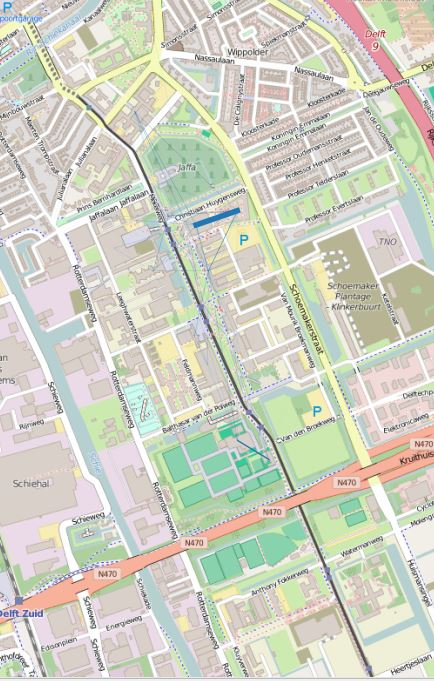
\includegraphics[scale=0.7]{pic2}
\captionsetup{justification=centering}
\caption{main window of GUI}
\label{figure:GUImain}
\end{figure}
To create a visualization, the user first has to select a time interval and then the buildings from and to which the movement should be visualized. The user has 2 options to select the time series for the current visualization: 
\begin{enumerate}
\item Click on '1. Add dates' which will open the date picker dialog
\item Pick a day from the dropdown menu and click on '2. All days of week' 
\end{enumerate}

\begin{figure}[H]
\captionsetup[subfigure]{justification=centering}
    \centering
    \begin{subfigure}[t]{0.5\textwidth}
        \centering
        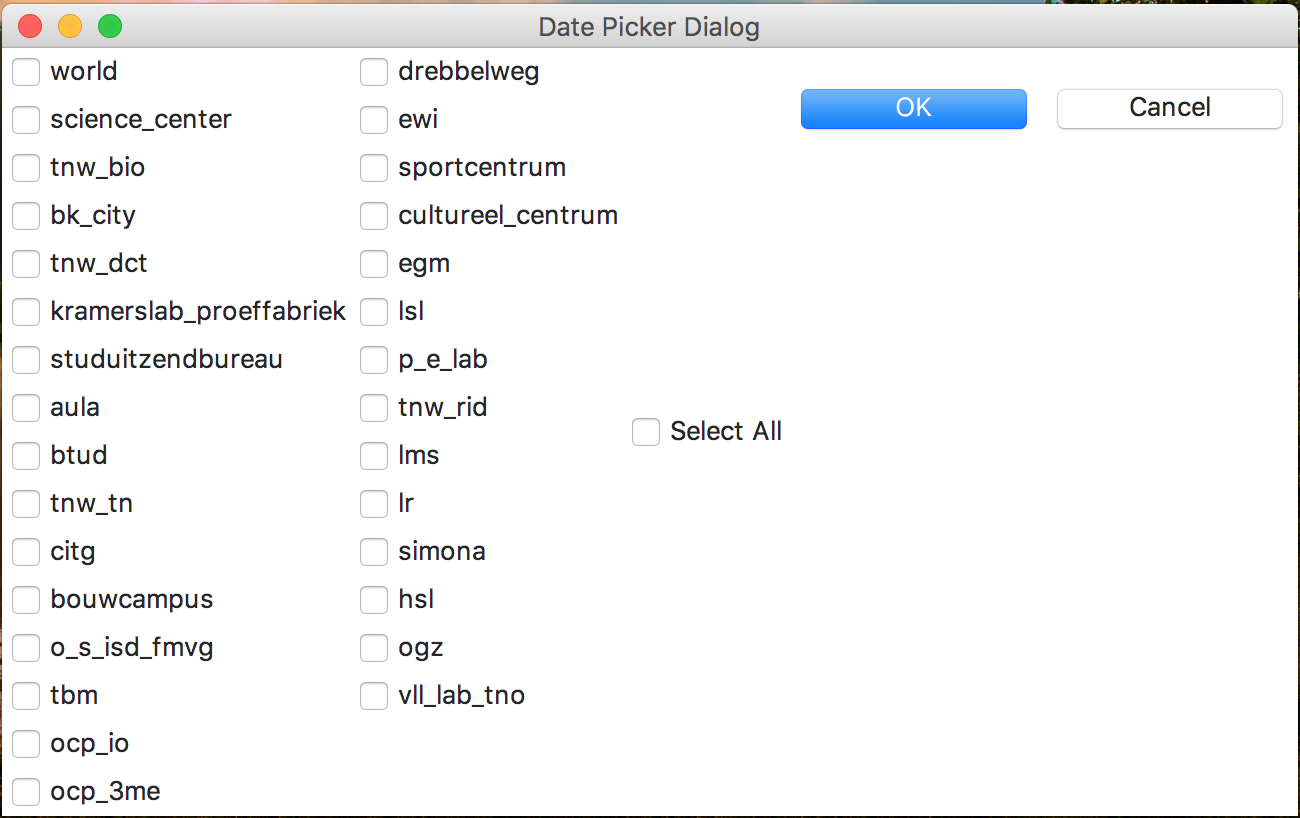
\includegraphics[scale=0.35]{GUI-buildings}
        \caption{buildings selection}
    \end{subfigure}%
    ~ 
    \begin{subfigure}[t]{0.5\textwidth}
        \centering
        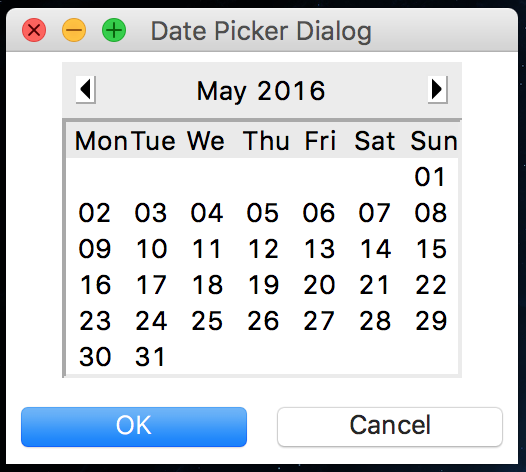
\includegraphics[scale=0.6]{GUI-dates}
        \caption{dates selection}
    \end{subfigure}
    \captionsetup{justification=centering}
    \caption{GUI selection windows}
    \label{figure:GUI selection}
\end{figure}

Option 1 can be used to select particular days without order. Option 2 can select 'every Tuesday' or even multiple recurring dates, such as 'every Monday to Friday'. It is also possible to combine option 1 and 2 to have for example 'every Monday and Friday the 13th of May'. 

After selecting the time series, the user has to select the buildings from and to which the movement should be visualized. The 3rd and 4th button bring up the same dialog. This dialog shows checkboxes for every building. Every building that is check will be visualized. The user also has the option to select all buildings. If the user would like to see movement from and to the same building, the user can select the same buildings twice.

\subsection{Bar chart}\label{barcharts}
\subsection{Maps}\label{maps}
In order to get an overview about how people move on the campus and further more,  find out movement patterns, a map visualization is essential. Map visualization consists of three parts: 
\begin{enumerate}
\item base map: open street map is used as base map. There are many labels on open street map, providing more context of the environment, so it is more clear and readable compared to other base maps like satellite images.
\item building markers: building markers show the locations of the buildings. Google maps marker style is used since it is commonly used in many map application. Because the shape of the building is not useful in analyzing movement patterns between buildings, each building is regarded as a point instead of a polygon, thus a node in the network, 
\item lines: lines are the most essential part in map visualization, they represent movements between buildings.
\end{enumerate}

In the first stage of map visualization, only base map and lines are taken into consideration, building markers are not shown on the map. The line width represents the amount of movement and movements are aggregated daily regardless of the timestamp of each movement during a day. This map visualization gives an overview of the movements over a day and between which buildings there are the most movements. The following maps show the difference of the amount of movement between April 11th (weekday) and April 17th (weekend).

\begin{figure}[H]
\captionsetup[subfigure]{justification=centering}
    \centering
    \begin{subfigure}[t]{0.5\textwidth}
        \centering
        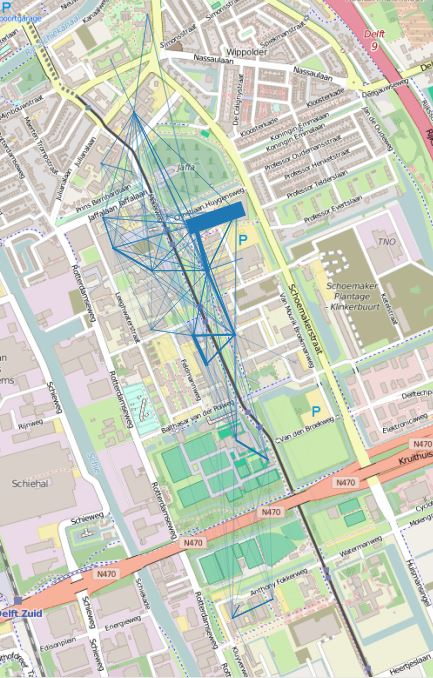
\includegraphics[scale=0.7]{pic1}
        \caption{April 11th, weekday}
    \end{subfigure}%
    ~ 
    \begin{subfigure}[t]{0.5\textwidth}
        \centering
        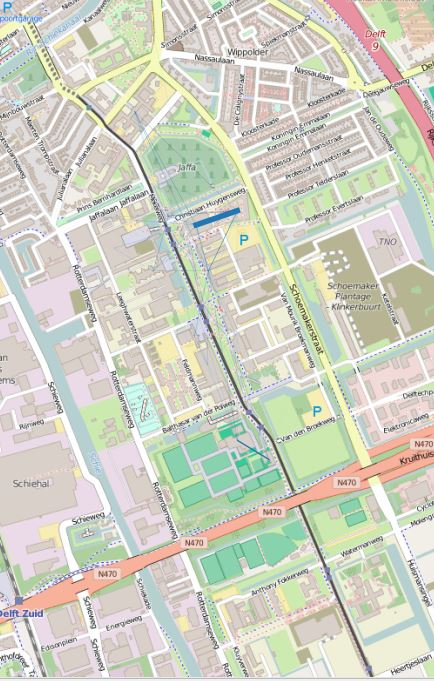
\includegraphics[scale=0.7]{pic2}
        \caption{April 17th, weekend}
    \end{subfigure}
    \captionsetup{justification=centering}
    \caption{Static visualization}
    \label{staticvisualization}
\end{figure}

It's clear that between Aula and library, there are the most movements and the amount of movements is totally different on weekday and on weekend.

Regarding the movements are dynamic and time is also highly related to movements, a dynamic map visualization is created to display individual movement over a day with temporal information. The following screenshots of the gif file show how the movements look like at a certain time of a day:

\begin{figure}[H]
\captionsetup[subfigure]{justification=centering}
    \centering
    \begin{subfigure}[t]{0.3\textwidth}
        \centering
        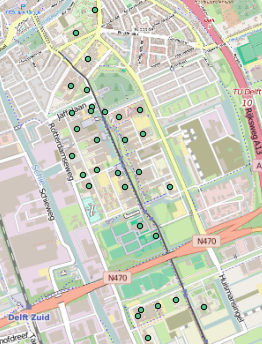
\includegraphics[scale=0.6]{frame009}
        \caption{7:00 am}
    \end{subfigure}%
    ~ 
    \begin{subfigure}[t]{0.3\textwidth}
        \centering
        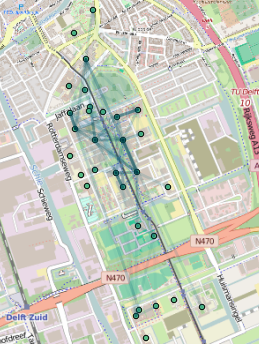
\includegraphics[scale=0.6]{frame021}
        \caption{9:00 am}
    \end{subfigure}
    \begin{subfigure}[t]{0.3\textwidth}
        \centering
        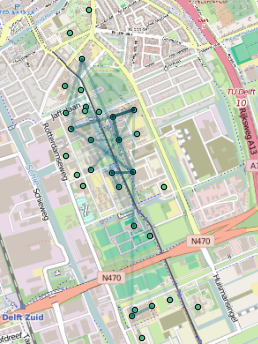
\includegraphics[scale=0.6]{frame033}
        \caption{11:00 am}
    \end{subfigure}
    \begin{subfigure}[t]{0.3\textwidth}
        \centering
        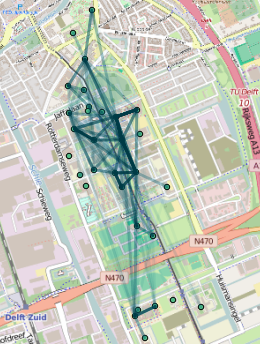
\includegraphics[scale=0.6]{frame045}
        \caption{13:00 pm}
    \end{subfigure}
    \begin{subfigure}[t]{0.3\textwidth}
        \centering
        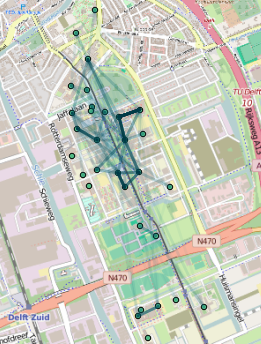
\includegraphics[scale=0.6]{frame057}
        \caption{15:00 pm}
    \end{subfigure}
    \begin{subfigure}[t]{0.3\textwidth}
        \centering
        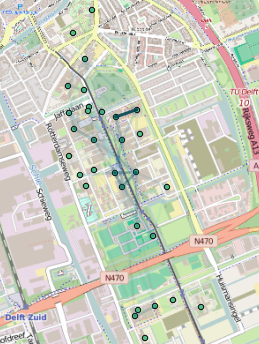
\includegraphics[scale=0.6]{frame066}
        \caption{16:30 pm}
    \end{subfigure}
    \begin{subfigure}[t]{0.3\textwidth}
        \centering
        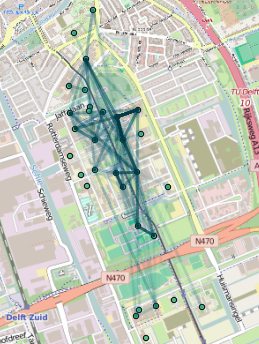
\includegraphics[scale=0.6]{frame075}
        \caption{18:00 pm}
    \end{subfigure}
    \begin{subfigure}[t]{0.3\textwidth}
        \centering
        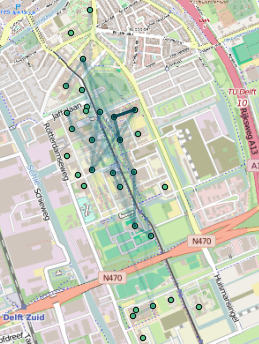
\includegraphics[scale=0.6]{frame087}
        \caption{20:00 pm}
    \end{subfigure}
    \begin{subfigure}[t]{0.3\textwidth}
        \centering
        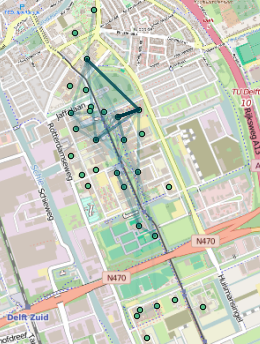
\includegraphics[scale=0.6]{frame099}
        \caption{22:00 pm}
    \end{subfigure}

    \captionsetup{justification=centering}
    \caption{Dynamic visualization of movements, April 11th}
    \label{autovisualization}
\end{figure}

In these pictures, the more movements there are, the less transparent the lines are. So generally speaking, from 7:00 am to 20:00 pm, there are two peaks at 13:00 pm and 18:00 pm. Hence, it is possible to get some insights about movement patterns from the animation. However, the dynamic map visualization doesn't provide detailed information to dig into but only an overview. So in order to mine on movement patterns, it is necessary to create maps containing more information, including time, direction and so forth. 

Because the amount of data is big, it is more convenient to generate maps automatically so that it will fasten the progress of finding movement patterns. According to the three components of map, there is some information needed to be collected before visualizing movement on map. The locations of buildings are collected manually on Google earth based the campus map. These locations are exported as KML file and imported into QGIS. After adding geometry columns x and y, the csv file is created and imported into database. By using $ST\_MakePoint$ function, a geometry column is created in database. In summary, the building locations are stored as the structure described in following table:

\begin{table}[H]
\centering
\begin{tabular}{|c|c|c|c|c|}
\hline 
id & name & geometry & x & y \\
\hline
0 & world & & & \\
\hline
3 & science\_ center & 010100000042A7.. & 4.36939919846287 & 52.0072322181367 \\
\hline
5 & tnw\_ bio & 010100000043AE.. & 4.37120211221402 & 52.0086132164098 \\
\hline
8 & bk\_ city & 010100000077E3.. & 4.37053698152436 & 52.0056562098059 \\
\hline
12 & tnw\_ dct & 01010000007CA.. & 4.36891378927259 & 52.0040834950037\\
\hline
.. & ... & ....& .... &....\\
\hline	
\end{tabular}
\captionsetup{justification=centering}
\caption{Building data structure}
\label{table:building}
\end{table}

There is a special 'building' called $world$ in the database. It is not an actual location, it is a virtual location which is used if someone is not scanned on the campus in a period of time. After storing the locations of buildings in the database, these locations will be extracted automatically from database to generate maps. There are two properties of lines used to deliver information:
\begin{enumerate}
\item width: line width is used to represent the amount of movements, but the amount is aggregated for both directions.
\item color: color is gradient from red to green. Red line means the movement is not symmetric that much more people move in one direction than the other, while green line means the movement is symmetric.
\end{enumerate}

Based on this map visualization, users can choose certain dates and certain buildings to generate maps automatically. It makes it easier to find out movement patterns. Since not all buildings are chosen, the map will only display the movements between several buildings, which makes the map more readable:

\begin{figure}[H]
	\centering
	\captionsetup[subfigure]{justification=centering}
	\begin{subfigure}[t]{0.48\textwidth}
	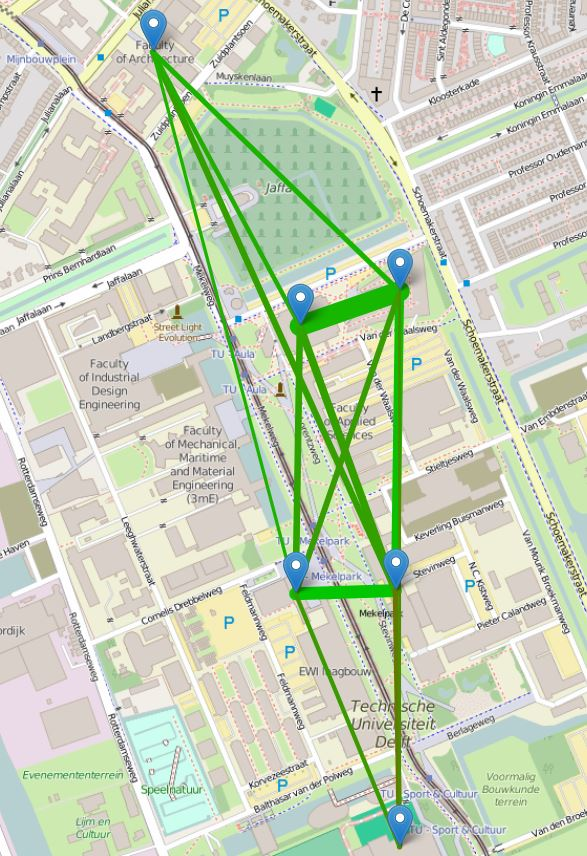
\includegraphics[scale=0.6]{pic3}
	\caption{Amount of movements on April 25th}
	\end{subfigure}
	\begin{subfigure}[t]{0.48\textwidth}
	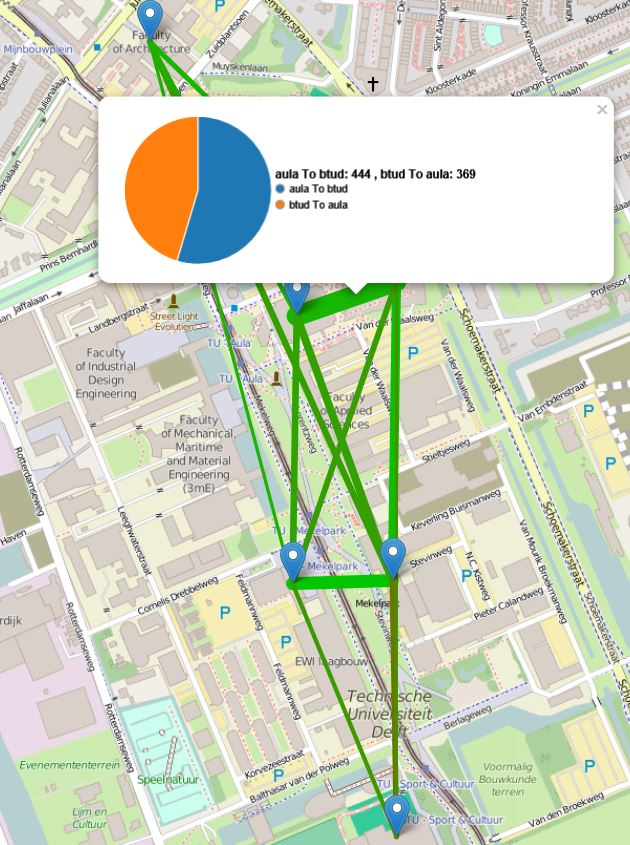
\includegraphics[scale=0.6]{pic4}
	\caption{Amount of movements in pie chart}
	\end{subfigure}
\end{figure}

As shown in the map, the lines are in different colors, which shows the symmetry of the movements. If the user is willing to know more about the movement, it is also possible to click on the line to check the amount of the movements for each direction in detail, and there will be a pie chart showing how symmetric the movements are. With the map visualization, it is easy to focus on movements which are special or interesting.

\section{Sequences}\label{sequences}
\subsection{introduction}
The following section describes how movement patterns were derived on campus level, without considering the direction of the movement. An association rule mining algorithm (Agrawal et al., 1993) was used to identify groups of buildings that frequently visited in combination with each other. Firstly the algorithm is described briefly, then the results are presented.
\subsection{Association rules mining}
Association rule mining is a technique to analyse what variables or items are commonly associated with each other in large databases. Probably the one of the main application is to analyse which items are commonly bought together by customers of a supermarket. As an example for this use case is an association rule of an itemset \{bread, butter\}, tells that in 80\% of those transactions including \{bread, butter\}, also \{milk\}  was present. In other words, 80\% of the people who buy bread and butter also buy milk (Agrawal et al., 1993). Compared to sequence mining, association rule mining does not consider the order of items neither within, nor across transactions.

Thus every rule is composed by two itemsets, the \textit{antecedent} \{bread,butter\} on the left-hand side, and the \textit{consequent} \{milk\} on the right-hand side. The rule is denoted as \{bread, butter\} \verb|=>| \{milk\}.

When a trajectory is simplified into a set of distinct buildings that the person
visited, association rules for buildings can be derived. In this case the rule
describes the set of buildings, or buildingset, that are commonly visited in
combination. For example the rule \{BK\_City, Aula\} \verb|=>| \{Library\}
tells that a group of people who visited the buildings BK\_City and Aula also
visited the Library.

As association rule mining does not consider the order of buildings, nor the
time spent in a building, it is important that these variables are appropriately
handled and noise is filtered out prior running the algorithm.

In the first version the buildingsets were stored in a table as below, where the
field \textit{mac} contains the mac-address of a device and each remaining field
represents a building. Value 1 is given if the device was recorded in a
building, otherwise no value is given. This binary encoding is rather simplistic
as it does not consider the amount of time spent in a building and therefore it
does not allow to differentiate between occasional or regular visits.

\begin{table}[H]
\centering
\captionsetup{justification=centering}
\caption{My caption}
\label{my-label}
\begin{tabular}{lllllll}
\cline{1-7}
mac & aula & bk\_city & bouwcampus & btud & ctig & ... \\ \cline{1-7}
A   & 1	& 1    	&        	&  	& 1	& 	\\
B   &  	&      	& 1      	& 1	&  	& 	\\
C   &  	& 1    	&        	&  	& 1	& 	\\
D   & 1	&      	&        	&  	&  	& 	\\
E   & 1	&      	& 1      	&  	&  	& 	\\ \cline{1-7}
\end{tabular}
\end{table}

Therefore in the second version a distinction between \textit{occasional,
regular} and \textit{frequent} stays was added to the buildingsets. The division
between the categories is based on the 40 hour workweek and 1.5 hour lecture
durations (Table X). 

\begin{table}[H]
\centering
\captionsetup{justification=centering}
\caption{My caption}
\label{my-label}
\begin{tabular}{lll}
\cline{1-3}
Category   & hours/week           	& ID \\ \cline{1-3}
occasional & $\leq 0.5$             	& 1  \\
regular	& $\textgreater 0.5, \leq 5$ & 2  \\
frequent   & $\textgreater 5$       	& 3
\end{tabular}
\end{table}

The trajectories of approximately 14,000 devices were used to create the first set of association rules with categorized stay duration. At this stage only the noise was filtered from the data but not the stationary devices, and people carrying two devices were not accounted for. The time range of trajectories spanned from 31.03.2016 to 02.05.2016, approximately one month.

Although there are several measures to evaluate the interestingness of an association rule  (Zhang et al., 2009), only \textit{support} and \textit{confidence} were used for testing purposes. 

\textbf{Support}
“The support for a rule is defined to be the fraction of transaction in the dataset that satisfy the union of items in the consequent and antecedent of the rule.” (Agrawal et al., 1993). In case of the rule \{BK\_City, Aula\} \verb|=>| \{Library\}, the support is the percentage of the total dataset that includes BK\_City, Aula and Library.

\textbf{Confidence}
Confidence measures the strength of the rule, and is considered as a conditional probability. In case of the rule \{BK\_ City, Aula\} \verb|=>| \{Library\}, the confidence is the probability that Library is in the trajectory if both BK\_ City and Aula are in the trajectory (Agrawal et al., 1993; Anbukkarasy \& Sairam, 2013).

The most interesting rules are displayed in \autoref{figure:buildingset}:
\begin{figure}[H]
\centering
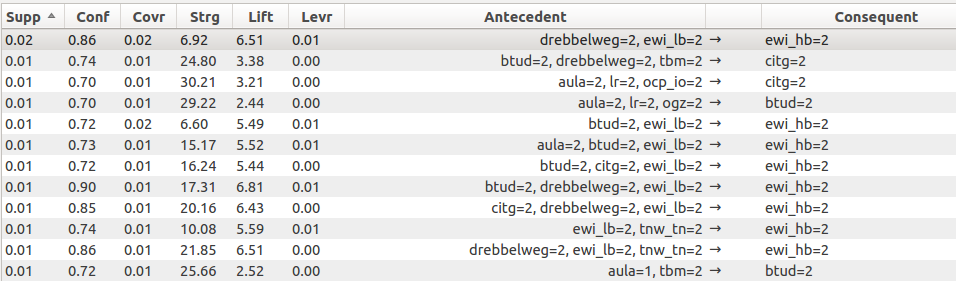
\includegraphics[scale=0.45]{acc_buildingset_v0516}
\captionsetup{justification=centering}
\caption{Amount of movements in pie chart}
\label{figure:buildingset}
\end{figure}

In the buildingset of approx. 14,000 devices 2\% was recorded in all of the buildings \textit{Drebbelweg, EWI-LB, EWI-HB} (Support = 0.02). There is an 86\% chance that if a device is recorded in the buildings \textit{Drebbelweg, EWI-LB}, then it is also recorded in \textit{EWI-HB} (Confidence = 0.86). And they spent on average between half hour to five hours a week in each building (drebbelweg=2, ewi\_ lb=2, ewi\_ hb=2).

\section{Pre-Processing}

Each chapter has its own file. For example, the \LaTeX{} source of this chapter can be found in \texttt{chapter-1.tex}. A chapter starts with the command
\begin{quote}
    \texttt{\textbackslash chapter\{Chapter title\}}
\end{quote}
This starts a new page, prints the chapter number and title and adds a link in the table of contents. If the title is very long, it may be desirable to use a shorter version in the page headers and the table of contents. This can be achieved by specifying the short title in brackets:
\begin{quote}
    \texttt{\textbackslash chapter[Short title]\{Very long title with many words which could not possibly fit on one line\}}
\end{quote}
Unnumbered chapters, such as the preface, can be created with \texttt{\textbackslash chapter*\{Chapter title\}}. Such a chapter will not show up in the table of contents or in the page header. To create a table of contents entry anyway, add
\begin{quote}
    \texttt{\textbackslash addcontentsline\{toc\}\{chapter\}\{Chapter title\}}
\end{quote}
after the \texttt{\textbackslash chapter} command. To print the chapter title in the page header, add
\begin{quote}
    \texttt{\textbackslash setheader\{Chapter title\}}
\end{quote}

Chapters are subdivided into sections, subsections, subsubsections, and, optionally, paragraphs and subparagraphs. All can have a title, but only sections and subsections are numbered. As with chapters, the numbering can be turned off by using \texttt{\textbackslash section*\{\ldots\}} instead of \texttt{\textbackslash section\{\ldots\}}, and similarly for the subsection.
\section{Entrances}\label{entrance}
\paragraph{\textbackslash paragraph\{\ldots\}}
Lorem ipsum dolor sit amet, consectetur adipisicing elit, sed do eiusmod tempor incididunt ut labore et dolore magna aliqua. Ut enim ad minim veniam, quis nostrud exercitation ullamco laboris nisi ut aliquip ex ea commodo consequat. Duis aute irure dolor in reprehenderit in voluptate velit esse cillum dolore eu fugiat nulla pariatur. Excepteur sint occaecat cupidatat non proident, sunt in culpa qui officia deserunt mollit anim id est laborum.

\section{Static and mobile devices}

The fonts used by this template depend on which version of \LaTeX{} you use. Regular \LaTeX, \emph{i.e.}, if you compile your document with with \texttt{latex}, \texttt{pslatex} or \texttt{pdflatex}, will use Utopia for text, Fourier for math and Latin Modern for sans-serif and monospaced text. 
However, if you want to adhere to the TU Delft house style, you will need to use \XeLaTeX, as it supports TrueType and OpenType fonts. Compiling with \texttt{xelatex} will use Arial for most titles and text, Courier New for monospace and Cambria for math. If you want to haf a sans-serif font for the
main text, while using \texttt{latex}, \texttt{pslatex} or \texttt{pdflatex}, you can use the option \texttt{noroman} in the report style: \texttt{\textbackslash usepackage[\ldots,noroman]{tudelft-report}}. For document and part titles,  TU Delft Ultra Light is used. For quotes, columns and text in boxes, you use Georgia. If you want to use \XeLaTeX, but do not want to use the TU Delft house style fonts, you can add the \texttt{nativefonts} option to the document class. This will still use  TU Delft Utra Light and Arial on the cover, but not for the body of the document. If you need to use these fonts for certain sections in the main text, they are available via \texttt{\textbackslash tudrmfamily} (Georgia) and \texttt{\textbackslash tudtitlefamily} (TU Delft Utra Light).

\begin{quote}
  You have to learn the rules of the game. And then you have to play better than anyone else.\\
  \emph{Albert Einstein}
\end{quote}

The corporate colors of the TU Delft are cyan, black and white, available via \texttt{\textbackslash color\{{\color{tudelft-cyan}tudelft-cyan}\}}, \texttt{\textbackslash color\{{\color{tudelft-black}tudelft-black}\}} (which differs slightly from the default \texttt{\textbackslash color\{black\}}) and \texttt{\textbackslash color\{tudelft-white\}}, respectively. Apart from these three, the house style defines the basic colors \texttt{\color{tudelft-sea-green}tudelft-sea-green}, \texttt{\color{tudelft-green}tudelft-green}, \texttt{\color{tudelft-dark-blue}tudelft-dark-blue}, \texttt{\color{tudelft-purple}tudelft-purple}, \texttt{\color{tudelft-turquoise}tudelft-turquoise} and \texttt{\color{tudelft-sky-blue}tudelft-sky-blue}, as well as the accent colors \texttt{\color{tudelft-lavendel}tudelft-lavendel}, \texttt{\color{tudelft-orange}tudelft-orange}, \texttt{\color{tudelft-warm-purple}tudelft-warm-purple}, \texttt{\color{tudelft-fuchsia}tudelft-fuchsia}, \texttt{\color{tudelft-bright-green}tudelft-bright-green} and \texttt{\color{tudelft-yellow}tudelft-yellow}.

